\documentclass{standalone}
\usepackage{ulem}
\usepackage{tikz}
\usepackage{caption}
\usepackage{subcaption}
\usetikzlibrary{positioning}

\title{sMDT Chamber Production at the University of Michigan}
\author{Evan Carpenter}
\date{February 7th, 2023}

\graphicspath{{./images}}

\definecolor{googlegreen}{rgb}{0.7137,0.8431,0.6588}
\definecolor{googleblue}{rgb}{0.4275,0.6196,0.9216}
\definecolor{googleyellow}{rgb}{1,1,0}
\definecolor{googlered}{rgb}{0.8784,0.4,0.4}


\def\ph{\textcolor{red}{PLACEHOLDER}}



\newcommand{\backupbegin}{
   \newcounter{finalframe}
   \setcounter{finalframe}{\value{framenumber}}
}
\newcommand{\backupend}{
   \setcounter{framenumber}{\value{finalframe}}
}
\begin{document}

	\begin{tikzpicture}
		\node at (0,0) {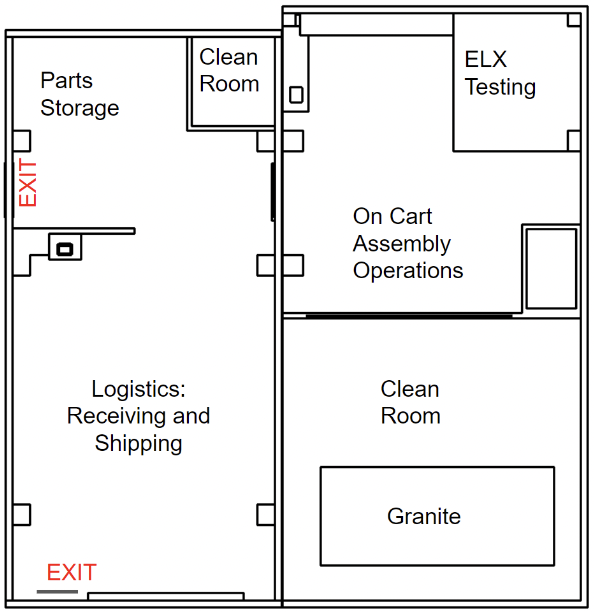
\includegraphics[width=0.3\pdfpagewidth]{HighBay.png}};
		\draw [help lines] (-4,-4)grid(4,4);
		\draw [ultra thick, googleyellow] (1.5,1.5)rectangle(3.25,3.25); % ELX rectangle
		%\draw [-latex, ultra thick, red] (1.1,2.425)--(1.5,2.425); % ELX arrow
		\draw [ultra thick, googlegreen] (0.1,-1.6)rectangle(2.9,-3); % granite rectangle
		%\draw [-latex, ultra thick, red] (0,-2.3)--(0.6,-2.3); % granite arrow
		\draw [ultra thick, googleblue] (0.5,0.2)rectangle(2,1.2); % on cart rectangle
		%\draw [-latex, ultra thick, red] (2.1,1.4)--(1.75,1); % on cart arrow
		%\node at (7,0) {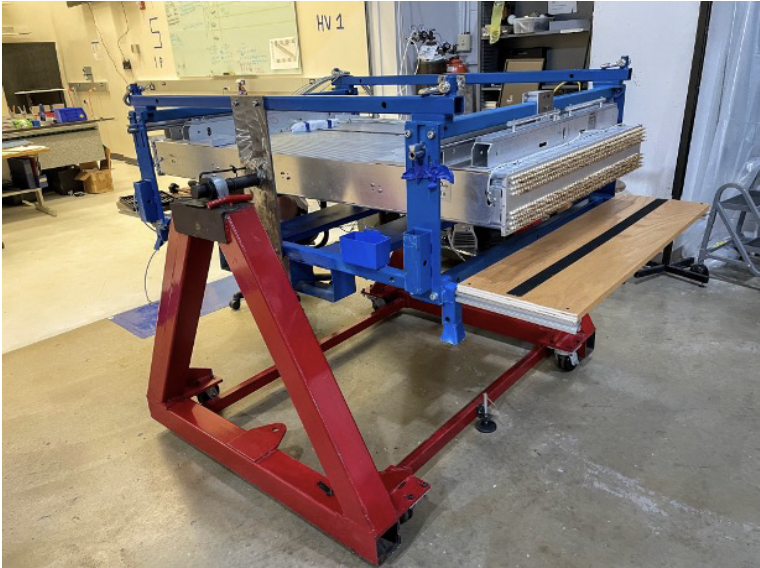
\includegraphics[width=0.3\pdfpagewidth]{OnRotationCart.png}};
		%\node at (7,6) {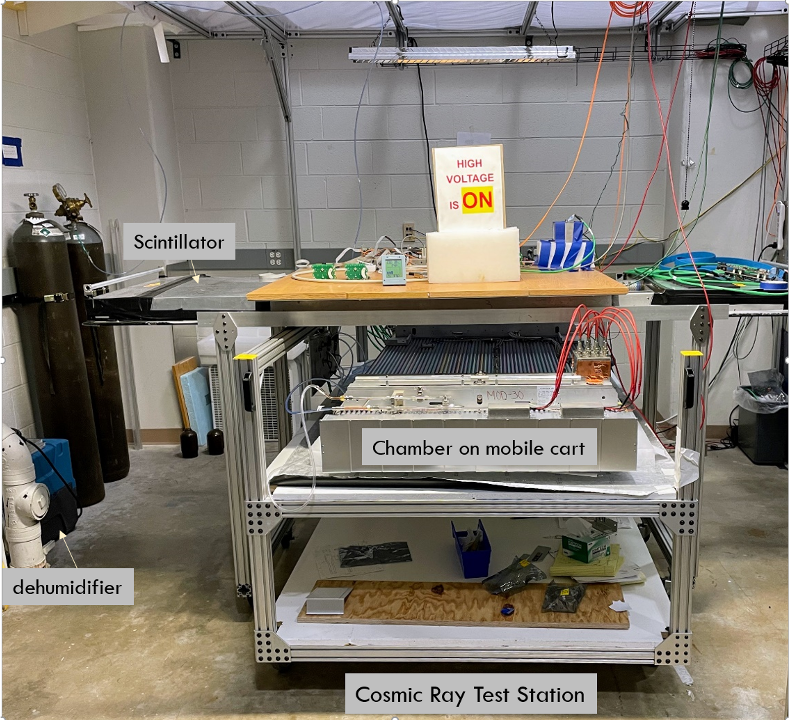
\includegraphics[width=0.3\pdfpagewidth]{CosmicRay-Station.png}};
		%\node at (3,-5.5) {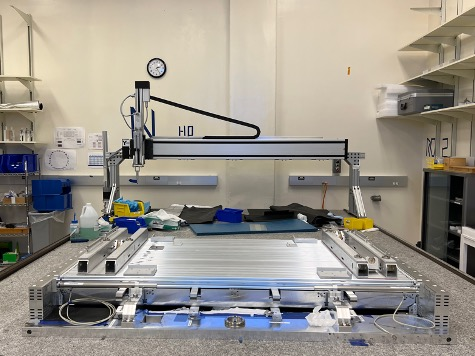
\includegraphics[width=0.3\pdfpagewidth]{Granite.png}};
	\end{tikzpicture}
\end{document}